%%%%%%%%%%%%%%%%%%%%%%%%%%%%%%%%%%%%%%%%%
% Beamer Presentation
% LaTeX Template
% Version 1.0 (10/11/12)
%
% This template has been downloaded from:
% http://www.LaTeXTemplates.com
%
% License:
% CC BY-NC-SA 3.0 (http://creativecommons.org/licenses/by-nc-sa/3.0/)
%
%%%%%%%%%%%%%%%%%%%%%%%%%%%%%%%%%%%%%%%%%

%----------------------------------------------------------------------------------------
%	PACKAGES AND THEMES
%----------------------------------------------------------------------------------------

\documentclass{beamer}

\mode<presentation> {

% The Beamer class comes with a number of default slide themes
% which change the colors and layouts of slides. Below this is a list
% of all the themes, uncomment each in turn to see what they look like.

%\usetheme{default}
%\usetheme{AnnArbor}
%\usetheme{Antibes}
%\usetheme{Bergen}
%\usetheme{Berkeley}
%\usetheme{Berlin}
%\usetheme{Boadilla}
%\usetheme{CambridgeUS}
%\usetheme{Copenhagen}
%\usetheme{Darmstadt}
%\usetheme{Dresden}
\usetheme{Frankfurt}
%\usetheme{Goettingen}
%\usetheme{Hannover}
%\usetheme{Ilmenau}
%\usetheme{JuanLesPins}
%\usetheme{Luebeck}
%\usetheme{Madrid}
%\usetheme{Malmoe}
%\usetheme{Marburg}
%\usetheme{Montpellier}
%\usetheme{PaloAlto}
%\usetheme{Pittsburgh}
%\usetheme{Rochester}
%\usetheme{Singapore}
%\usetheme{Szeged}
%\usetheme{Warsaw}

% As well as themes, the Beamer class has a number of color themes
% for any slide theme. Uncomment each of these in turn to see how it
% changes the colors of your current slide theme.

%\usecolortheme{albatross}
%\usecolortheme{beaver}
%\usecolortheme{beetle}
%\usecolortheme{crane}
%\usecolortheme{dolphin}
%\usecolortheme{dove}
%\usecolortheme{fly}
%\usecolortheme{lily}
%\usecolortheme{orchid}
%\usecolortheme{rose}
%\usecolortheme{seagull}
%\usecolortheme{seahorse}
\usecolortheme{whale}
%\usecolortheme{wolverine}

%\setbeamertemplate{footline} % To remove the footer line in all slides uncomment this line
%\setbeamertemplate{footline}[page number] % To replace the footer line in all slides with a simple slide count uncomment this line

%\setbeamertemplate{navigation symbols}{} % To remove the navigation symbols from the bottom of all slides uncomment this line
}

\usepackage{graphicx} % Allows including images
\usepackage{booktabs} % Allows the use of \toprule, \midrule and \bottomrule in tables

%----------------------------------------------------------------------------------------
%	TITLE PAGE
%----------------------------------------------------------------------------------------

\title[Short title]{Git,Github:Don't get scared,Get started } % The short title appears at the bottom of every slide, the full title is only on the title page

\author{Rosni K V} % Your name
\institute[FOSS cell] % Your institution as it will appear on the bottom of every slide, may be shorthand to save space
{
Govt. Engg College , Sreekrishnapuram \\ % Your institution for the title page
\medskip
\textit{rosnikv@gmail.com} % Your email address
}
\date{\today} % Date, can be changed to a custom date

\begin{document}

\begin{frame}
\titlepage % Print the title page as the first slide
\begin{center}
 
\includegraphics[scale=0.1]{GitHub.jpg}
\end{center}
\end{frame}

\begin{frame}
\frametitle{Overview}% Table of contents slide, comment this block out to remove it
%\includegraphics[scale=0.5]{images/myimage.jpg}
\tableofcontents % Throughout your presentation, if you choose to use \section{} and \subsection{} commands, these will automatically be printed on this slide as an overview of your presentation
\end{frame}

%----------------------------------------------------------------------------------------
%	PRESENTATION SLIDES
%----------------------------------------------------------------------------------------

%------------------------------------------------
\section{Git and github} % Sections can be created in order to organize your presentation into discrete blocks, all sections and subsections are automatically printed in the table of contents as an overview of the talk
%------------------------------------------------

\subsection{Git} % A subsection can be created just before a set of slides with a common theme to further break down your presentation into chunks

\begin{frame}
\frametitle{Heard about git ?}
\begin{itemize}
 \item \textbf{Git is a free and open source distributed version control system.}
 \item It is a version control system means that it can help you keep track of files that are frequently changed.
\end{itemize}
\begin{center}
  
\includegraphics[scale=0.25]{socialite.jpg}
\end{center}
\end{frame}
%------------------------------------------------
\subsection{Git architecture}
\begin{frame}
\frametitle{Git architecture}
  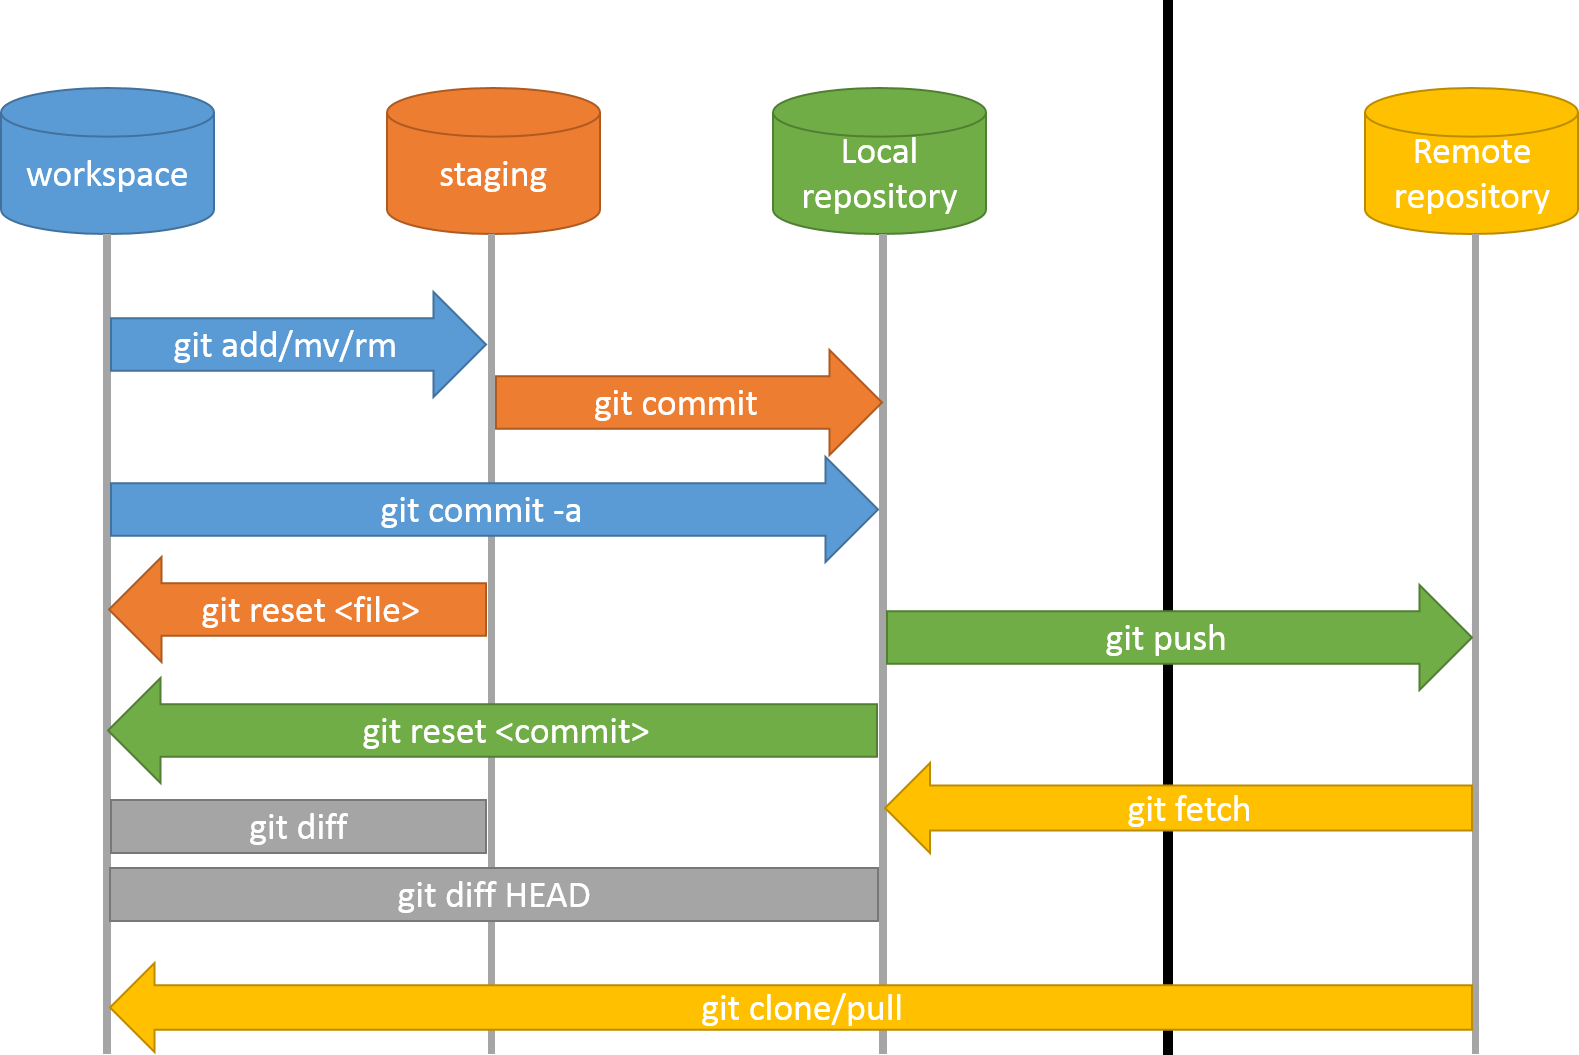
\includegraphics[scale=0.4]{git-remote.png}
\end{frame}

\subsection{git workflow}
\begin{frame}
\frametitle{Git architecture}

\begin{block}{Workflow}
\text The basic Git workflow goes something like this: 
\begin{itemize}
 \item You modify files in your working directory.
 \item You stage the files, adding snapshots of them to your staging area.
 \item You do a commit, which takes the files as they are in the staging area and stores that snapshot permanently to your Git directory. 
\end{itemize}

\end{block}
\end{frame}
%------------------------------------------------
\subsection{Github}
\begin{frame}
\frametitle{What about Github ?}
\begin{itemize}
\item \textbf{GitHub is an amazing service.}
  
\includegraphics[scale=0.1]{github_client.png}
\item GitHub is a web-based service for people who want to use git.
\item It’s widely used by teams who want to make some or all of their work publicly available under an open source license.
\item Since that’s what we do, we feel that GitHub is a natural choice for us to store our code.
\item it's a social network that has completely changed the way we work :)
\end{itemize}
\end{frame}


%------------------------------------------------


%------------------------------------------------
\section{Get started social coding !}
%------------------------------------------------
\subsection{How to get started ?}
\begin{frame}
\frametitle{How to get started ?}
\begin{figure}
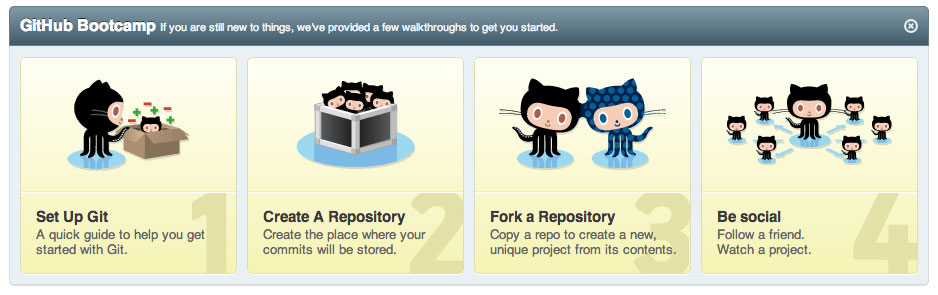
\includegraphics[width=1.1\linewidth]{original}
\end{figure}
\end{frame}

\subsection{Terminology}
\begin{frame}
\frametitle{Words People Use When They Talk About Git}
\begin{columns}[c] % The "c" option specifies centered vertical alignment while the "t" option is used for top vertical alignment

\column{.45\textwidth} % Left column and width
%\textbf{Heading}
\begin{enumerate}
\item Command Line
\item Repository
\item Version Control
\item Commit
\item Branch
\end{enumerate}

\column{.5\textwidth} % Right column and width
%Lorem ipsum dolor sit amet, consectetur adipiscing elit. Integer lectus nisl, ultricies in feugiat rutrum, porttitor sit amet augue. Aliquam ut tortor mauris. Sed volutpat ante purus, quis accumsan dolor.
\begin{figure}

\includegraphics[width=1.1\linewidth]{terms}
\end{figure}
\end{columns}
\end{frame}

\subsection{Some commands}
\begin{frame}
\frametitle{some commands}
\begin{columns}[c] % The "c" option specifies centered vertical alignment while the "t" option is used for top vertical alignment

\column{.45\textwidth} % Left column and width
\textbf{Getting a Repository}
\vspace{1cm}
\begin{enumerate}
\item git init
\item git clone
\end{enumerate}
\vspace{1cm}
\textbf{Commits}
\vspace{1cm}
\begin{enumerate}
\item git add
\item git commit
\end{enumerate}

\column{.5\textwidth} % Right column and width
%Lorem ipsum dolor sit amet, consectetur adipiscing elit. Integer lectus nisl, ultricies in feugiat rutrum, porttitor sit amet augue. Aliquam ut tortor mauris. Sed volutpat ante purus, quis accumsan dolor.
\textbf{Getting information}
\vspace{1cm}
\begin{enumerate}
\item git help
\item git status
\item git diff
\item git log
\item git show
\end{enumerate}
\end{columns}
\end{frame}

\subsection{Setting up git and github}
\begin{frame}
\frametitle{Setting up git and github}
\begin{itemize}
\item \textbf{Make yourself a \textit{GitHub account} first.}
\vspace{1cm}
  
\includegraphics[scale=0.2]{set.png}
\end{itemize}
\end{frame}

\begin{frame}
\frametitle{Setting up git and github}
\begin{itemize}
\item \textbf{And install \textit{git} in your system}
\vspace{1cm}
  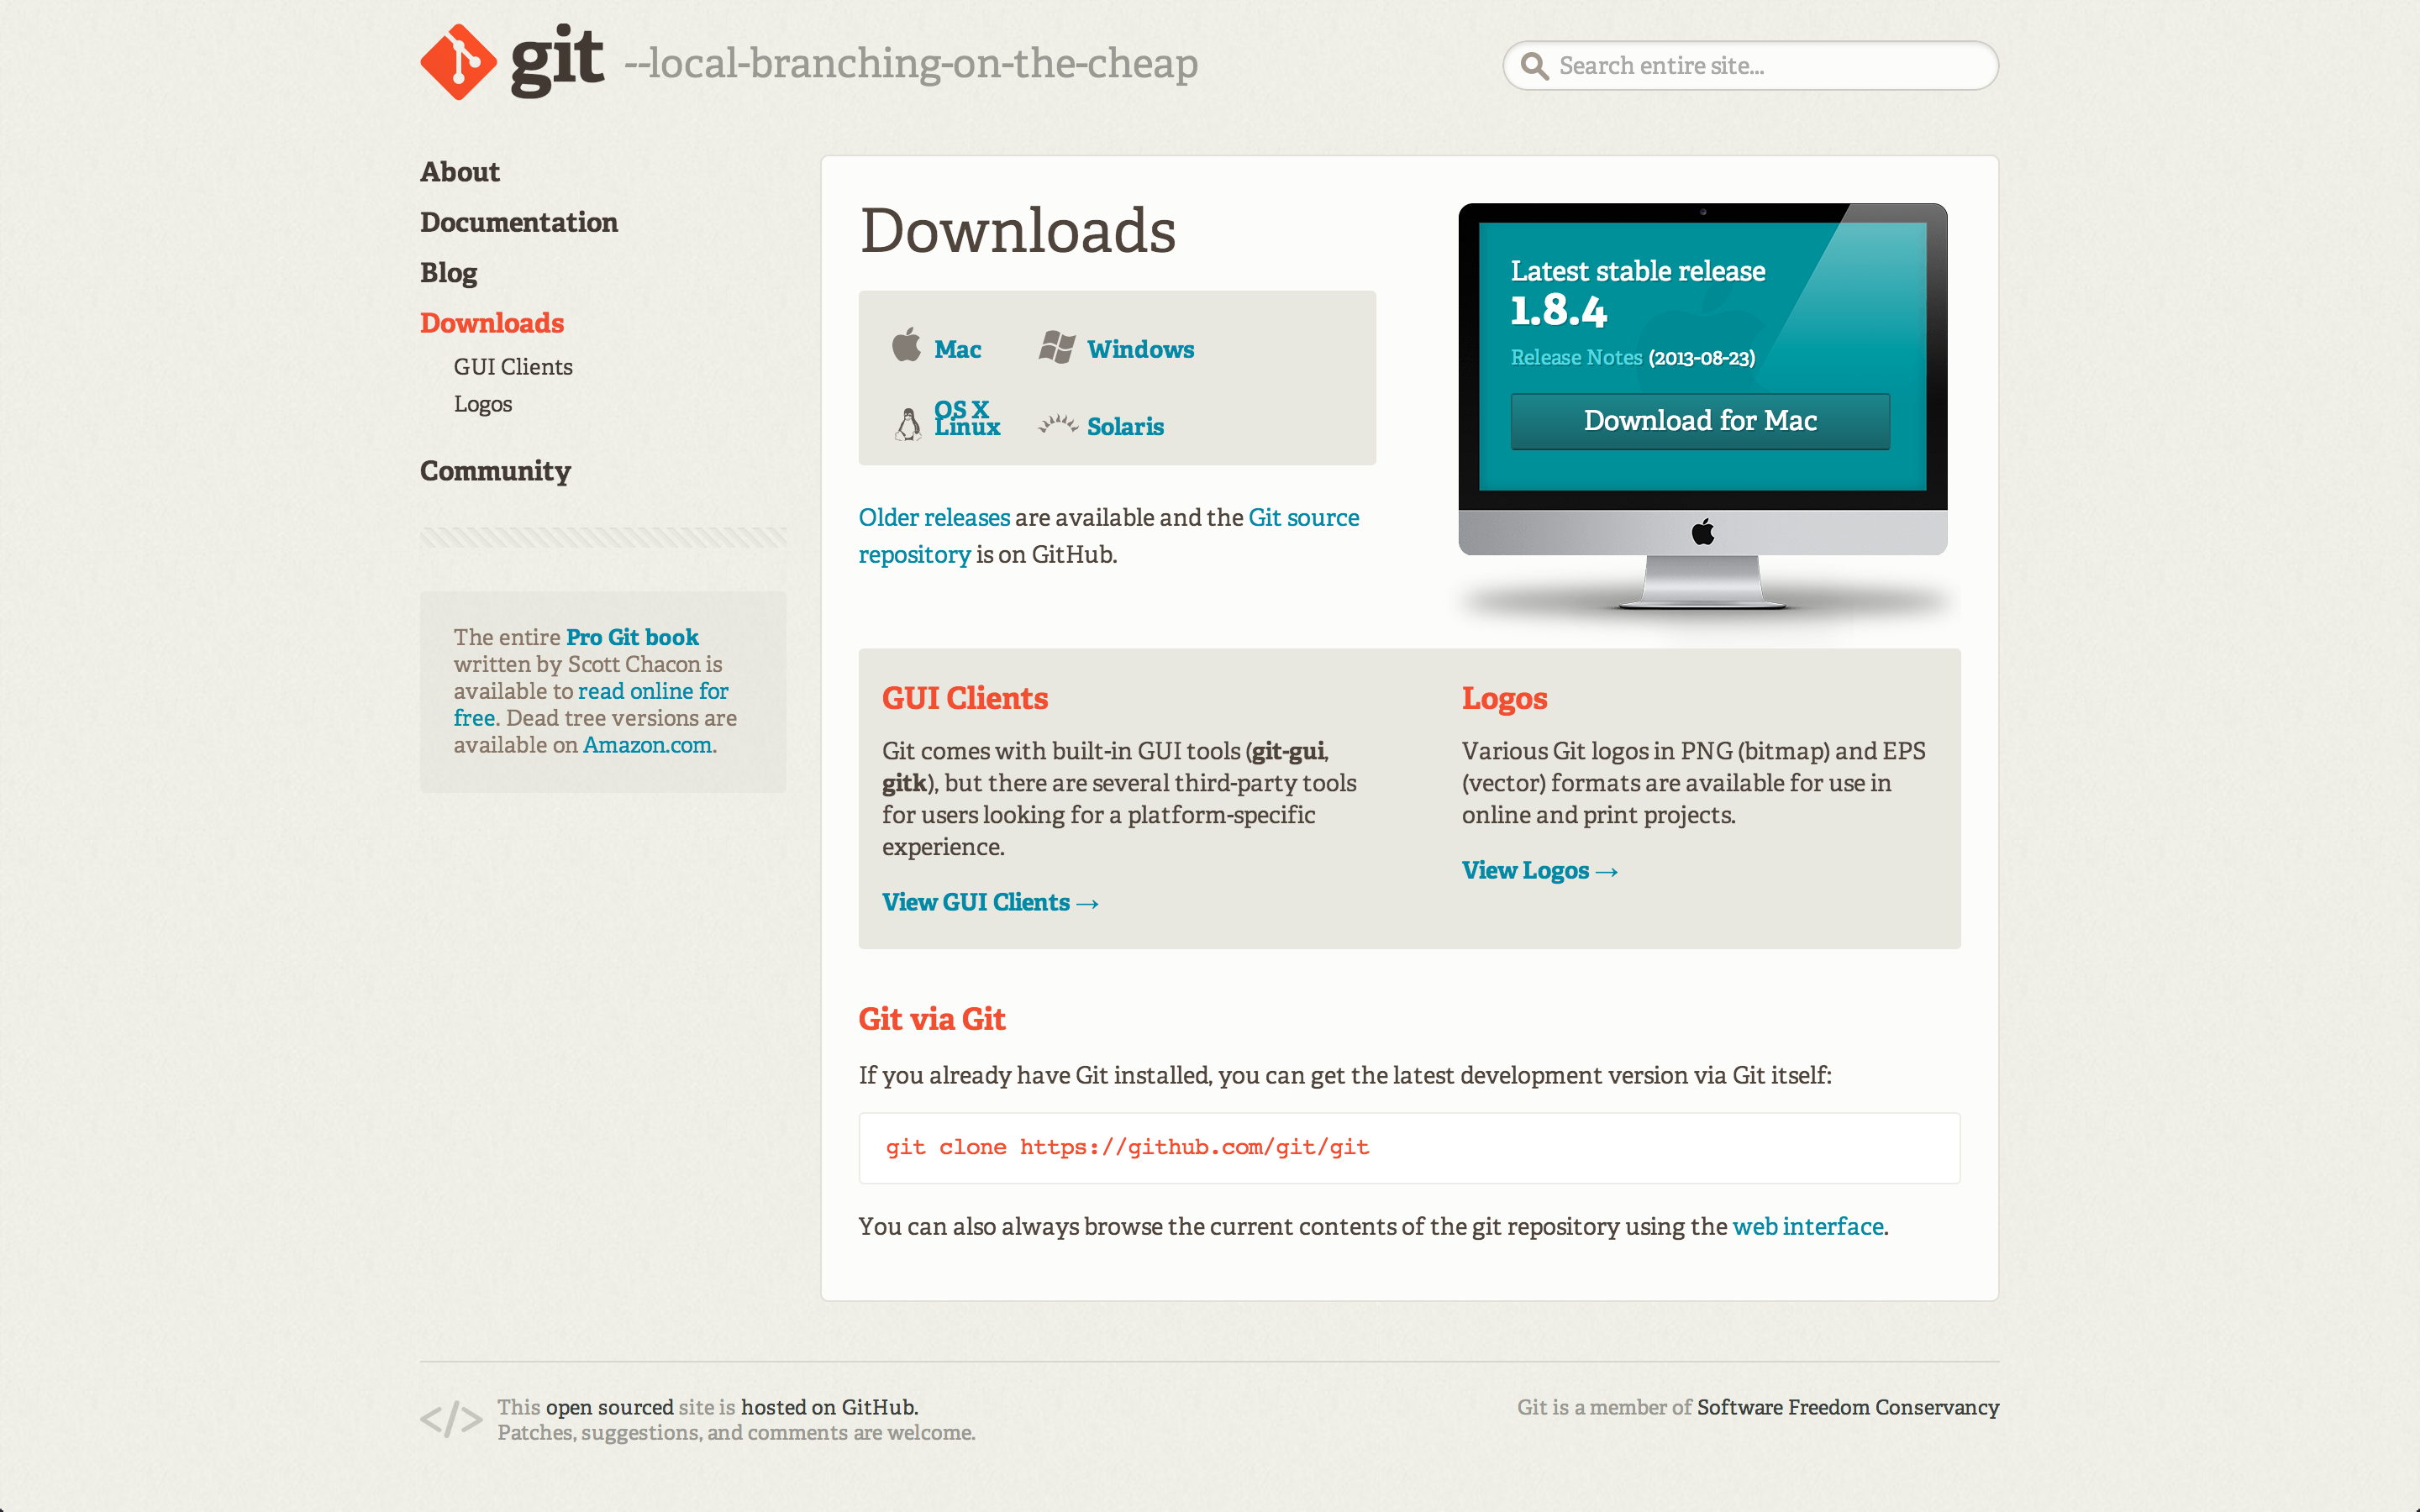
\includegraphics[scale=0.2]{setup.png}
\end{itemize}
\end{frame}
  
\subsection{Try these...}
\begin{frame}
\frametitle{Try some specific commands}
\begin{columns}[c] % The "c" option specifies centered vertical alignment while the "t" option is used for top vertical alignment
\column{.45\textwidth} % Left column and width
%
\includegraphics[scale=0.3]{tryit.jpg}
\begin{enumerate}
\item git init
\item git config
\item git help
\item git status
\item git add
\item git commit
\end{enumerate}

\column{.5\textwidth} % Right column and width
%Lorem ipsum dolor sit amet, consectetur adipiscing elit. Integer lectus nisl, ultricies in feugiat rutrum, porttitor sit amet augue. Aliquam ut tortor mauris. Sed volutpat ante purus, quis accumsan dolor.
\begin{enumerate}
\item git branch
\item git checkout
\item git merge
\item git push
\item git pull
\end{enumerate}
\end{columns}
\end{frame}

\subsection{Working with git}
\begin{frame}
\frametitle{Working with git}
\textbf{first git commands !}
\vspace{1cm}
\newline
\textit {git config --global user.name "Your Name Here"}
\newline
\textit {git config --global user.email "your\_email$@$youremail.com"}
\newline
\end{frame}

\subsection{Our first git repo}
\begin{frame}
\frametitle{Our first git repo}
\textbf{Create new repo from your github page,it is the online repository...}
  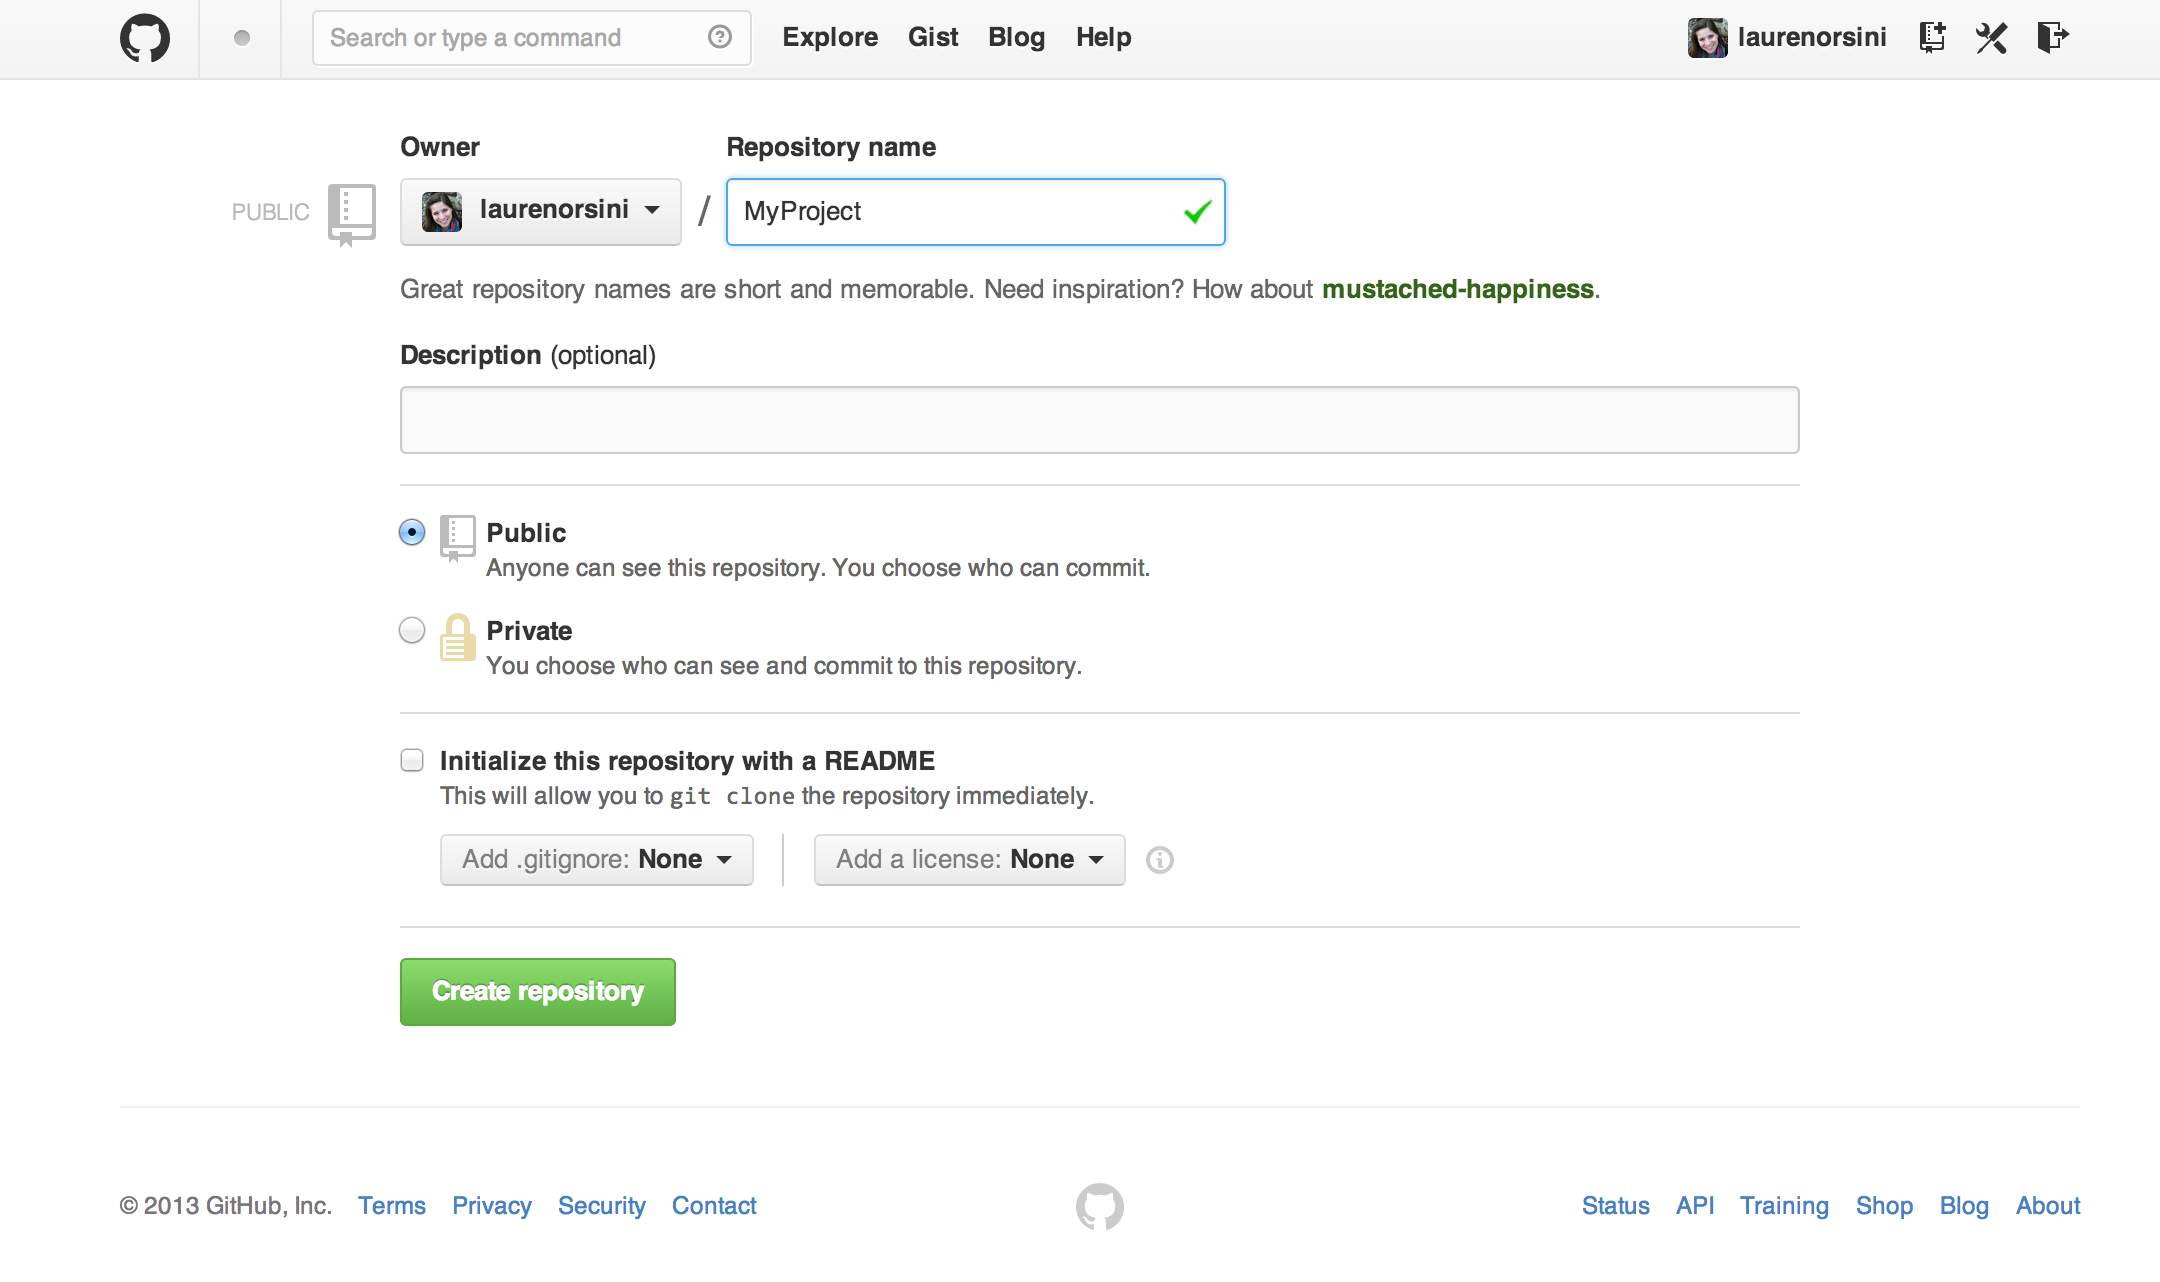
\includegraphics[scale=0.25]{newrepo.png}
\end{frame}

\begin{frame}
\frametitle{Our first git repo}
\textbf{Now create the local repository...}
\vspace{1cm}
\begin{itemize}
 \item mkdir /home/user/MyProject
 \item cd /home/user/MyProject
 \item git init 
\end{itemize}
\small
\text If you already had a repository ready to go, you'd just need to cd to that directory and then run the git init command in there instead.
\newline
\newline
\text Run this command to create a README file:  \textit{touch README}
\end{frame}

\begin{frame}
\frametitle{Our first git repo}
\begin{itemize}
 \item git add README
 \text Now, run this command to commit it:
 \item git commit -m 'first commit'
 \text To get this empty README file to GitHub, you need to push it with a couple of commands.
 \item git remote add origin https://github.com/yourusername/Hello-World.github
 \item git push origin master
\end{itemize}
\end{frame}

\begin{frame}
\frametitle{ Congratulations on your first commit!}
%Uncomment the code on this slide to include your own image from the same directory as the template .TeX file.

\includegraphics[scale=0.8]{ydi.jpg}
\end{frame}

\begin{frame}
\frametitle{ Check codeschool<> to explore and learn more about git.}
%Uncomment the code on this slide to include your own image from the same directory as the template .TeX file.

\includegraphics[scale=0.2]{codeschool.png}
\end{frame}
%\begin{frame}
%\frametitle{Table}
%\begin{table}
%\begin{tabular}{l l l}
%\toprule
%\textbf{Treatments} & \textbf{Response 1} & \textbf{Response 2}\\
%\midrule
%Treatment 1 & 0.0003262 & 0.562 \\
%Treatment 2 & 0.0015681 & 0.910 \\
%Treatment 3 & 0.0009271 & 0.296 \\
%\bottomrule
%\end{tabular}
%\caption{Table caption}
%\end{table}
%\end{frame}

%------------------------------------------------

%\begin{frame}
%\frametitle{Theorem}
%\begin{theorem}[Mass--energy equivalence]
%$E = mc^2$
%\end{theorem}
%\end{frame}

%------------------------------------------------

%\begin{frame}[fragile] % Need to use the fragile option when verbatim is used in the slide
%\frametitle{Verbatim}
%\begin{example}[Theorem Slide Code]
%\begin{verbatim}
%\begin{frame}
%\frametitle{Theorem}
%\begin{theorem}[Mass--energy equivalence]
%$E = mc^2$
%\end{theorem}
%\end{frame}\end{verbatim}
%\end{example}
%\end{frame}

%------------------------------------------------

%\begin{frame}
%\frametitle{Figure}
%Uncomment the code on this slide to include your own image from the same directory as the template .TeX file.
%\begin{figure}
%\includegraphics[width=0.8\linewidth]{test}
%\end{figure}
%\end{frame}

%------------------------------------------------

%\begin{frame}[fragile] % Need to use the fragile option when verbatim is used in the slide
%\frametitle{Citation}
%An example of the \verb|\cite| command to cite within the presentation:\\~

%This statement requires citation \cite{p1}.
%\end{frame}

%------------------------------------------------

%\begin{frame}
%\frametitle{References}
%\footnotesize{
%\begin{thebibliography}{99} % Beamer does not support BibTeX so references must be inserted manually as below
%\bibitem[Smith, 2012]{p1} John Smith (2012)
%\newblock Title of the publication
%\newblock \emph{Journal Name} 12(3), 45 -- 678.
%\end{thebibliography}
%}
%\end{frame}

%------------------------------------------------

\begin{frame}
\Huge{\centerline{Have fun managing your code!}}
\end{frame}

%----------------------------------------------------------------------------------------

\end{document} 